%% ===============================================
\begin{subfigure}[b]{0.14\textwidth}
\caption{\label{fig:16nn}}
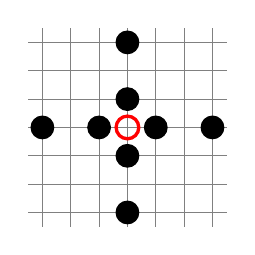
\begin{tikzpicture}[scale=0.36]
\draw[step=1,color=gray] (-3.5,-3.5) grid (3.5,3.5);
\draw[very thick,red] (0, 0) circle (.4);
%%\ draw[very thick] (0,0) circle (2);
%% 1
\filldraw[black] (0,-1) circle (.4);
\filldraw[black] (0,+1) circle (.4);
\filldraw[black] (-1,0) circle (.4);
\filldraw[black] (+1,0) circle (.4);
%% 6
\filldraw[black] (0,-3) circle (.4);
\filldraw[black] (0,+3) circle (.4);
\filldraw[black] (-3,0) circle (.4);
\filldraw[black] (+3,0) circle (.4);
\end{tikzpicture}
\end{subfigure}
%% ===============================================
\hfill
%% ===============================================
\begin{subfigure}[b]{0.14\textwidth}
\caption{\label{fig:26nn}}
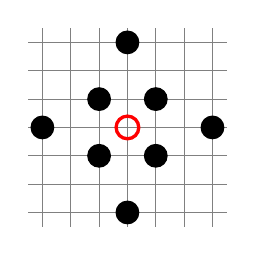
\begin{tikzpicture}[scale=0.36]
\draw[step=1,color=gray] (-3.5,-3.5) grid (3.5,3.5);
\draw[very thick,red] (0, 0) circle (.4);
%%\ draw[very thick] (0,0) circle (2);
%% 2
\filldraw[black] (+1,-1) circle (.4);
\filldraw[black] (+1,+1) circle (.4);
\filldraw[black] (-1,-1) circle (.4);
\filldraw[black] (-1,+1) circle (.4);
%% 6
\filldraw[black] (0,-3) circle (.4);
\filldraw[black] (0,+3) circle (.4);
\filldraw[black] (-3,0) circle (.4);
\filldraw[black] (+3,0) circle (.4);
\end{tikzpicture}
\end{subfigure}
%% ===============================================
\hfill
%% ===============================================
\begin{subfigure}[b]{0.14\textwidth}
\caption{\label{fig:36nn}}
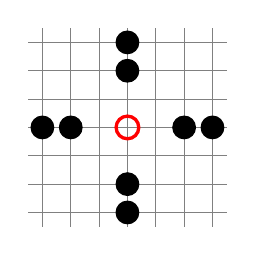
\begin{tikzpicture}[scale=0.36]
\draw[step=1,color=gray] (-3.5,-3.5) grid (3.5,3.5);
\draw[very thick,red] (0, 0) circle (.4);
%%\ draw[very thick] (0,0) circle (2);
%% 3
\filldraw[black] ( 0,-2) circle (.4);
\filldraw[black] ( 0,+2) circle (.4);
\filldraw[black] (-2, 0) circle (.4);
\filldraw[black] (+2, 0) circle (.4);
%% 6
\filldraw[black] (0,-3) circle (.4);
\filldraw[black] (0,+3) circle (.4);
\filldraw[black] (-3,0) circle (.4);
\filldraw[black] (+3,0) circle (.4);
\end{tikzpicture}
\end{subfigure}
%% ===============================================
\hfill
%% ===============================================
\begin{subfigure}[b]{0.14\textwidth}
\caption{\label{fig:46nn}}
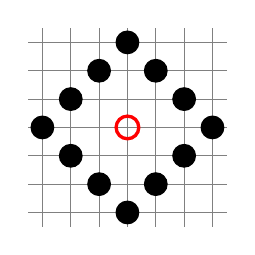
\begin{tikzpicture}[scale=0.36]
\draw[step=1,color=gray] (-3.5,-3.5) grid (3.5,3.5);
\draw[very thick,red] (0, 0) circle (.4);
%%\ draw[very thick] (0,0) circle (2);
%% 4
\filldraw[black] (-2,-1) circle (.4);
\filldraw[black] (-2,+1) circle (.4);
\filldraw[black] (-1,-2) circle (.4);
\filldraw[black] (-1,+2) circle (.4);
\filldraw[black] (+1,-2) circle (.4);
\filldraw[black] (+1,+2) circle (.4);
\filldraw[black] (+2,-1) circle (.4);
\filldraw[black] (+2,+1) circle (.4);
%% 6
\filldraw[black] (0,-3) circle (.4);
\filldraw[black] (0,+3) circle (.4);
\filldraw[black] (-3,0) circle (.4);
\filldraw[black] (+3,0) circle (.4);
\end{tikzpicture}
\end{subfigure}
%% ===============================================
\hfill
%% ===============================================
\begin{subfigure}[b]{0.14\textwidth}
\caption{\label{fig:56nn}}
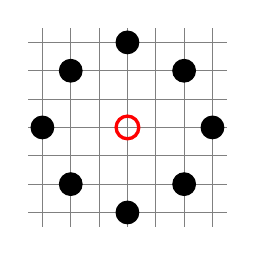
\begin{tikzpicture}[scale=0.36]
\draw[step=1,color=gray] (-3.5,-3.5) grid (3.5,3.5);
\draw[very thick,red] (0, 0) circle (.4);
%%\ draw[very thick] (0,0) circle (2);
%% 5
\filldraw[black] (-2,-2) circle (.4);
\filldraw[black] (-2,+2) circle (.4);
\filldraw[black] (+2,-2) circle (.4);
\filldraw[black] (+2,+2) circle (.4);
%% 6
\filldraw[black] (0,-3) circle (.4);
\filldraw[black] (0,+3) circle (.4);
\filldraw[black] (-3,0) circle (.4);
\filldraw[black] (+3,0) circle (.4);
\end{tikzpicture}
\end{subfigure}
%% ===============================================
\hfill
%% ===============================================
\begin{subfigure}[b]{0.14\textwidth}
\caption{\label{fig:126nn}}
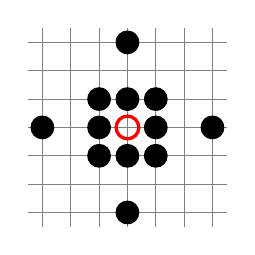
\begin{tikzpicture}[scale=0.36]
\draw[step=1,color=gray] (-3.5,-3.5) grid (3.5,3.5);
\draw[very thick,red] (0, 0) circle (.4);
%%\ draw[very thick] (0,0) circle (2);
%% 1
\filldraw[black] (0,-1) circle (.4);
\filldraw[black] (0,+1) circle (.4);
\filldraw[black] (-1,0) circle (.4);
\filldraw[black] (+1,0) circle (.4);
%% 2
\filldraw[black] (+1,-1) circle (.4);
\filldraw[black] (+1,+1) circle (.4);
\filldraw[black] (-1,-1) circle (.4);
\filldraw[black] (-1,+1) circle (.4);
%% 6
\filldraw[black] (0,-3) circle (.4);
\filldraw[black] (0,+3) circle (.4);
\filldraw[black] (-3,0) circle (.4);
\filldraw[black] (+3,0) circle (.4);
\end{tikzpicture}
\end{subfigure}
%% ===============================================
\hfill
%% ===============================================
\begin{subfigure}[b]{0.14\textwidth}
\caption{\label{fig:136nn}}
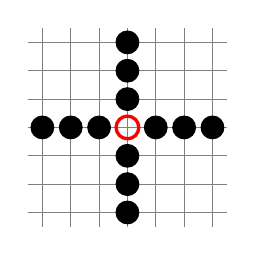
\begin{tikzpicture}[scale=0.36]
\draw[step=1,color=gray] (-3.5,-3.5) grid (3.5,3.5);
\draw[very thick,red] (0, 0) circle (.4);
%%\ draw[very thick] (0,0) circle (2);
%% 1
\filldraw[black] (0,-1) circle (.4);
\filldraw[black] (0,+1) circle (.4);
\filldraw[black] (-1,0) circle (.4);
\filldraw[black] (+1,0) circle (.4);
%% 3
\filldraw[black] ( 0,-2) circle (.4);
\filldraw[black] ( 0,+2) circle (.4);
\filldraw[black] (-2, 0) circle (.4);
\filldraw[black] (+2, 0) circle (.4);
%% 6
\filldraw[black] (0,-3) circle (.4);
\filldraw[black] (0,+3) circle (.4);
\filldraw[black] (-3,0) circle (.4);
\filldraw[black] (+3,0) circle (.4);
\end{tikzpicture}
\end{subfigure}
%% ===============================================
\hfill
%% ===============================================
\begin{subfigure}[b]{0.14\textwidth}
\caption{\label{fig:146nn}}
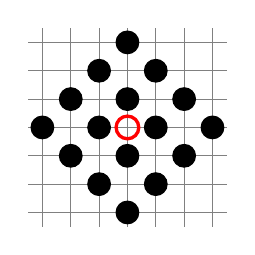
\begin{tikzpicture}[scale=0.36]
\draw[step=1,color=gray] (-3.5,-3.5) grid (3.5,3.5);
\draw[very thick,red] (0, 0) circle (.4);
%%\ draw[very thick] (0,0) circle (2);
%% 1
\filldraw[black] (0,-1) circle (.4);
\filldraw[black] (0,+1) circle (.4);
\filldraw[black] (-1,0) circle (.4);
\filldraw[black] (+1,0) circle (.4);
%% 4
\filldraw[black] (-2,-1) circle (.4);
\filldraw[black] (-2,+1) circle (.4);
\filldraw[black] (-1,-2) circle (.4);
\filldraw[black] (-1,+2) circle (.4);
\filldraw[black] (+1,-2) circle (.4);
\filldraw[black] (+1,+2) circle (.4);
\filldraw[black] (+2,-1) circle (.4);
\filldraw[black] (+2,+1) circle (.4);
%% 6
\filldraw[black] (0,-3) circle (.4);
\filldraw[black] (0,+3) circle (.4);
\filldraw[black] (-3,0) circle (.4);
\filldraw[black] (+3,0) circle (.4);
\end{tikzpicture}
\end{subfigure}
%% ===============================================
\hfill
%% ===============================================
\begin{subfigure}[b]{0.14\textwidth}
\caption{\label{fig:156nn}}
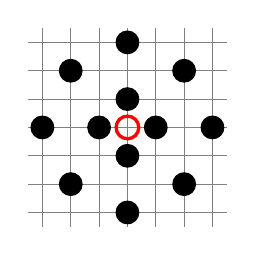
\begin{tikzpicture}[scale=0.36]
\draw[step=1,color=gray] (-3.5,-3.5) grid (3.5,3.5);
\draw[very thick,red] (0, 0) circle (.4);
%%\ draw[very thick] (0,0) circle (2);
%% 1
\filldraw[black] (0,-1) circle (.4);
\filldraw[black] (0,+1) circle (.4);
\filldraw[black] (-1,0) circle (.4);
\filldraw[black] (+1,0) circle (.4);
%% 5
\filldraw[black] (-2,-2) circle (.4);
\filldraw[black] (-2,+2) circle (.4);
\filldraw[black] (+2,-2) circle (.4);
\filldraw[black] (+2,+2) circle (.4);
%% 6
\filldraw[black] (0,-3) circle (.4);
\filldraw[black] (0,+3) circle (.4);
\filldraw[black] (-3,0) circle (.4);
\filldraw[black] (+3,0) circle (.4);
\end{tikzpicture}
\end{subfigure}
%% ===============================================
\hfill
%% ===============================================
\begin{subfigure}[b]{0.14\textwidth}
\caption{\label{fig:236nn}}
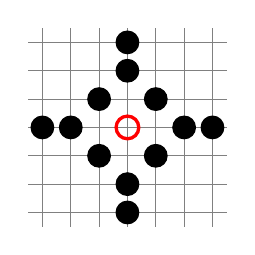
\begin{tikzpicture}[scale=0.36]
\draw[step=1,color=gray] (-3.5,-3.5) grid (3.5,3.5);
\draw[very thick,red] (0, 0) circle (.4);
%%\ draw[very thick] (0,0) circle (2);
%% 2
\filldraw[black] (+1,-1) circle (.4);
\filldraw[black] (+1,+1) circle (.4);
\filldraw[black] (-1,-1) circle (.4);
\filldraw[black] (-1,+1) circle (.4);
%% 3
\filldraw[black] ( 0,-2) circle (.4);
\filldraw[black] ( 0,+2) circle (.4);
\filldraw[black] (-2, 0) circle (.4);
\filldraw[black] (+2, 0) circle (.4);
%% 6
\filldraw[black] (0,-3) circle (.4);
\filldraw[black] (0,+3) circle (.4);
\filldraw[black] (-3,0) circle (.4);
\filldraw[black] (+3,0) circle (.4);
\end{tikzpicture}
\end{subfigure}
%% ===============================================
\hfill
%% ===============================================
\begin{subfigure}[b]{0.14\textwidth}
\caption{\label{fig:246nn}}
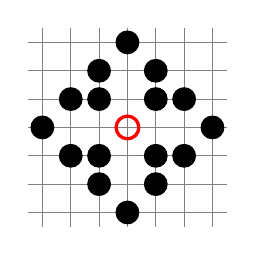
\begin{tikzpicture}[scale=0.36]
\draw[step=1,color=gray] (-3.5,-3.5) grid (3.5,3.5);
\draw[very thick,red] (0, 0) circle (.4);
%%\ draw[very thick] (0,0) circle (2);
%% 2
\filldraw[black] (+1,-1) circle (.4);
\filldraw[black] (+1,+1) circle (.4);
\filldraw[black] (-1,-1) circle (.4);
\filldraw[black] (-1,+1) circle (.4);
%% 4
\filldraw[black] (-2,-1) circle (.4);
\filldraw[black] (-2,+1) circle (.4);
\filldraw[black] (-1,-2) circle (.4);
\filldraw[black] (-1,+2) circle (.4);
\filldraw[black] (+1,-2) circle (.4);
\filldraw[black] (+1,+2) circle (.4);
\filldraw[black] (+2,-1) circle (.4);
\filldraw[black] (+2,+1) circle (.4);
%% 6
\filldraw[black] (0,-3) circle (.4);
\filldraw[black] (0,+3) circle (.4);
\filldraw[black] (-3,0) circle (.4);
\filldraw[black] (+3,0) circle (.4);
\end{tikzpicture}
\end{subfigure}
%% ===============================================
\hfill
%% ===============================================
\begin{subfigure}[b]{0.14\textwidth}
\caption{\label{fig:256nn}}
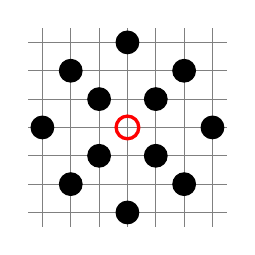
\begin{tikzpicture}[scale=0.36]
\draw[step=1,color=gray] (-3.5,-3.5) grid (3.5,3.5);
\draw[very thick,red] (0, 0) circle (.4);
%%\ draw[very thick] (0,0) circle (2);
%% 2
\filldraw[black] (+1,-1) circle (.4);
\filldraw[black] (+1,+1) circle (.4);
\filldraw[black] (-1,-1) circle (.4);
\filldraw[black] (-1,+1) circle (.4);
%% 5
\filldraw[black] (-2,-2) circle (.4);
\filldraw[black] (-2,+2) circle (.4);
\filldraw[black] (+2,-2) circle (.4);
\filldraw[black] (+2,+2) circle (.4);
%% 6
\filldraw[black] (0,-3) circle (.4);
\filldraw[black] (0,+3) circle (.4);
\filldraw[black] (-3,0) circle (.4);
\filldraw[black] (+3,0) circle (.4);
\end{tikzpicture}
\end{subfigure}
%% ===============================================
\hfill
%% ===============================================
\begin{subfigure}[b]{0.14\textwidth}
\caption{\label{fig:346nn}}
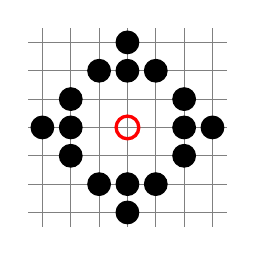
\begin{tikzpicture}[scale=0.36]
\draw[step=1,color=gray] (-3.5,-3.5) grid (3.5,3.5);
\draw[very thick,red] (0, 0) circle (.4);
%%\ draw[very thick] (0,0) circle (2);
%% 3
\filldraw[black] ( 0,-2) circle (.4);
\filldraw[black] ( 0,+2) circle (.4);
\filldraw[black] (-2, 0) circle (.4);
\filldraw[black] (+2, 0) circle (.4);
%% 4
\filldraw[black] (-2,-1) circle (.4);
\filldraw[black] (-2,+1) circle (.4);
\filldraw[black] (-1,-2) circle (.4);
\filldraw[black] (-1,+2) circle (.4);
\filldraw[black] (+1,-2) circle (.4);
\filldraw[black] (+1,+2) circle (.4);
\filldraw[black] (+2,-1) circle (.4);
\filldraw[black] (+2,+1) circle (.4);
%% 6
\filldraw[black] (0,-3) circle (.4);
\filldraw[black] (0,+3) circle (.4);
\filldraw[black] (-3,0) circle (.4);
\filldraw[black] (+3,0) circle (.4);
\end{tikzpicture}
\end{subfigure}
%% ===============================================
\hfill
%% ===============================================
\begin{subfigure}[b]{0.14\textwidth}
\caption{\label{fig:356nn}}
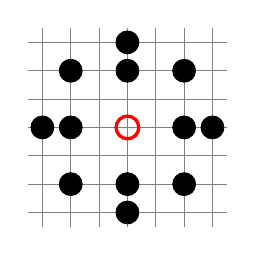
\begin{tikzpicture}[scale=0.36]
\draw[step=1,color=gray] (-3.5,-3.5) grid (3.5,3.5);
\draw[very thick,red] (0, 0) circle (.4);
%%\ draw[very thick] (0,0) circle (2);
%% 3
\filldraw[black] ( 0,-2) circle (.4);
\filldraw[black] ( 0,+2) circle (.4);
\filldraw[black] (-2, 0) circle (.4);
\filldraw[black] (+2, 0) circle (.4);
%% 5
\filldraw[black] (-2,-2) circle (.4);
\filldraw[black] (-2,+2) circle (.4);
\filldraw[black] (+2,-2) circle (.4);
\filldraw[black] (+2,+2) circle (.4);
%% 6
\filldraw[black] (0,-3) circle (.4);
\filldraw[black] (0,+3) circle (.4);
\filldraw[black] (-3,0) circle (.4);
\filldraw[black] (+3,0) circle (.4);
\end{tikzpicture}
\end{subfigure}
%% ===============================================
\hfill
%% ===============================================
\begin{subfigure}[b]{0.14\textwidth}
\caption{\label{fig:456nn}}
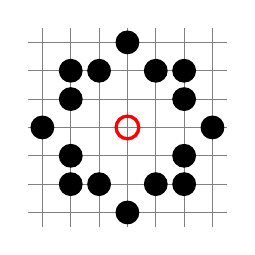
\begin{tikzpicture}[scale=0.36]
\draw[step=1,color=gray] (-3.5,-3.5) grid (3.5,3.5);
\draw[very thick,red] (0, 0) circle (.4);
%%\ draw[very thick] (0,0) circle (2);
%% 4
\filldraw[black] (-2,-1) circle (.4);
\filldraw[black] (-2,+1) circle (.4);
\filldraw[black] (-1,-2) circle (.4);
\filldraw[black] (-1,+2) circle (.4);
\filldraw[black] (+1,-2) circle (.4);
\filldraw[black] (+1,+2) circle (.4);
\filldraw[black] (+2,-1) circle (.4);
\filldraw[black] (+2,+1) circle (.4);
%% 5
\filldraw[black] (-2,-2) circle (.4);
\filldraw[black] (-2,+2) circle (.4);
\filldraw[black] (+2,-2) circle (.4);
\filldraw[black] (+2,+2) circle (.4);
%% 6
\filldraw[black] (0,-3) circle (.4);
\filldraw[black] (0,+3) circle (.4);
\filldraw[black] (-3,0) circle (.4);
\filldraw[black] (+3,0) circle (.4);
\end{tikzpicture}
\end{subfigure}
%% ===============================================
\hfill
%% ===============================================
\begin{subfigure}[b]{0.14\textwidth}
\caption{\label{fig:1236nn}}
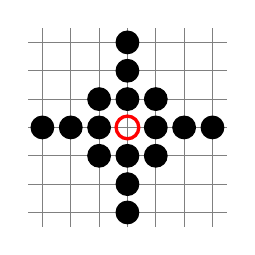
\begin{tikzpicture}[scale=0.36]
\draw[step=1,color=gray] (-3.5,-3.5) grid (3.5,3.5);
\draw[very thick,red] (0, 0) circle (.4);
%%\ draw[very thick] (0,0) circle (2);
%% 1
\filldraw[black] (0,-1) circle (.4);
\filldraw[black] (0,+1) circle (.4);
\filldraw[black] (-1,0) circle (.4);
\filldraw[black] (+1,0) circle (.4);
%% 2
\filldraw[black] (+1,-1) circle (.4);
\filldraw[black] (+1,+1) circle (.4);
\filldraw[black] (-1,-1) circle (.4);
\filldraw[black] (-1,+1) circle (.4);
%% 3
\filldraw[black] ( 0,-2) circle (.4);
\filldraw[black] ( 0,+2) circle (.4);
\filldraw[black] (-2, 0) circle (.4);
\filldraw[black] (+2, 0) circle (.4);
%% 6
\filldraw[black] (0,-3) circle (.4);
\filldraw[black] (0,+3) circle (.4);
\filldraw[black] (-3,0) circle (.4);
\filldraw[black] (+3,0) circle (.4);
\end{tikzpicture}
\end{subfigure}
%% ===============================================
\hfill
%% ===============================================
\begin{subfigure}[b]{0.14\textwidth}
\caption{\label{fig:1246nn}}
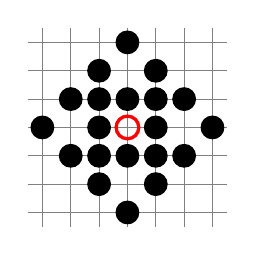
\begin{tikzpicture}[scale=0.36]
\draw[step=1,color=gray] (-3.5,-3.5) grid (3.5,3.5);
\draw[very thick,red] (0, 0) circle (.4);
%%\ draw[very thick] (0,0) circle (2);
%% 1
\filldraw[black] (0,-1) circle (.4);
\filldraw[black] (0,+1) circle (.4);
\filldraw[black] (-1,0) circle (.4);
\filldraw[black] (+1,0) circle (.4);
%% 2
\filldraw[black] (+1,-1) circle (.4);
\filldraw[black] (+1,+1) circle (.4);
\filldraw[black] (-1,-1) circle (.4);
\filldraw[black] (-1,+1) circle (.4);
%% 4
\filldraw[black] (-2,-1) circle (.4);
\filldraw[black] (-2,+1) circle (.4);
\filldraw[black] (-1,-2) circle (.4);
\filldraw[black] (-1,+2) circle (.4);
\filldraw[black] (+1,-2) circle (.4);
\filldraw[black] (+1,+2) circle (.4);
\filldraw[black] (+2,-1) circle (.4);
\filldraw[black] (+2,+1) circle (.4);
%% 6
\filldraw[black] (0,-3) circle (.4);
\filldraw[black] (0,+3) circle (.4);
\filldraw[black] (-3,0) circle (.4);
\filldraw[black] (+3,0) circle (.4);
\end{tikzpicture}
\end{subfigure}
%% ===============================================
\hfill
%% ===============================================
\begin{subfigure}[b]{0.14\textwidth}
\caption{\label{fig:1256nn}}
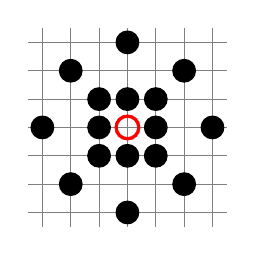
\begin{tikzpicture}[scale=0.36]
\draw[step=1,color=gray] (-3.5,-3.5) grid (3.5,3.5);
\draw[very thick,red] (0, 0) circle (.4);
%%\ draw[very thick] (0,0) circle (2);
%% 1
\filldraw[black] (0,-1) circle (.4);
\filldraw[black] (0,+1) circle (.4);
\filldraw[black] (-1,0) circle (.4);
\filldraw[black] (+1,0) circle (.4);
%% 2
\filldraw[black] (+1,-1) circle (.4);
\filldraw[black] (+1,+1) circle (.4);
\filldraw[black] (-1,-1) circle (.4);
\filldraw[black] (-1,+1) circle (.4);
%% 5
\filldraw[black] (-2,-2) circle (.4);
\filldraw[black] (-2,+2) circle (.4);
\filldraw[black] (+2,-2) circle (.4);
\filldraw[black] (+2,+2) circle (.4);
%% 6
\filldraw[black] (0,-3) circle (.4);
\filldraw[black] (0,+3) circle (.4);
\filldraw[black] (-3,0) circle (.4);
\filldraw[black] (+3,0) circle (.4);
\end{tikzpicture}
\end{subfigure}
%% ===============================================
\hfill
%% ===============================================
\begin{subfigure}[b]{0.14\textwidth}
\caption{\label{fig:1346nn}}
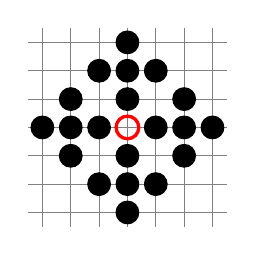
\begin{tikzpicture}[scale=0.36]
\draw[step=1,color=gray] (-3.5,-3.5) grid (3.5,3.5);
\draw[very thick,red] (0, 0) circle (.4);
%%\ draw[very thick] (0,0) circle (2);
%% 1
\filldraw[black] (0,-1) circle (.4);
\filldraw[black] (0,+1) circle (.4);
\filldraw[black] (-1,0) circle (.4);
\filldraw[black] (+1,0) circle (.4);
%% 3
\filldraw[black] ( 0,-2) circle (.4);
\filldraw[black] ( 0,+2) circle (.4);
\filldraw[black] (-2, 0) circle (.4);
\filldraw[black] (+2, 0) circle (.4);
%% 4
\filldraw[black] (-2,-1) circle (.4);
\filldraw[black] (-2,+1) circle (.4);
\filldraw[black] (-1,-2) circle (.4);
\filldraw[black] (-1,+2) circle (.4);
\filldraw[black] (+1,-2) circle (.4);
\filldraw[black] (+1,+2) circle (.4);
\filldraw[black] (+2,-1) circle (.4);
\filldraw[black] (+2,+1) circle (.4);
%% 6
\filldraw[black] (0,-3) circle (.4);
\filldraw[black] (0,+3) circle (.4);
\filldraw[black] (-3,0) circle (.4);
\filldraw[black] (+3,0) circle (.4);
\end{tikzpicture}
\end{subfigure}
%% ===============================================
\hfill
%% ===============================================
\begin{subfigure}[b]{0.14\textwidth}
\caption{\label{fig:1356nn}}
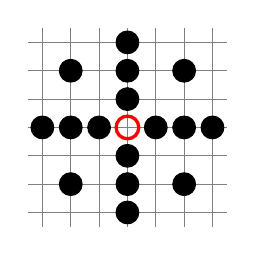
\begin{tikzpicture}[scale=0.36]
\draw[step=1,color=gray] (-3.5,-3.5) grid (3.5,3.5);
\draw[very thick,red] (0, 0) circle (.4);
%%\ draw[very thick] (0,0) circle (2);
%% 1
\filldraw[black] (0,-1) circle (.4);
\filldraw[black] (0,+1) circle (.4);
\filldraw[black] (-1,0) circle (.4);
\filldraw[black] (+1,0) circle (.4);
%% 3
\filldraw[black] ( 0,-2) circle (.4);
\filldraw[black] ( 0,+2) circle (.4);
\filldraw[black] (-2, 0) circle (.4);
\filldraw[black] (+2, 0) circle (.4);
%% 5
\filldraw[black] (-2,-2) circle (.4);
\filldraw[black] (-2,+2) circle (.4);
\filldraw[black] (+2,-2) circle (.4);
\filldraw[black] (+2,+2) circle (.4);
%% 6
\filldraw[black] (0,-3) circle (.4);
\filldraw[black] (0,+3) circle (.4);
\filldraw[black] (-3,0) circle (.4);
\filldraw[black] (+3,0) circle (.4);
\end{tikzpicture}
\end{subfigure}
%% ===============================================
\hfill
%% ===============================================
\begin{subfigure}[b]{0.14\textwidth}
\caption{\label{fig:1456nn}}
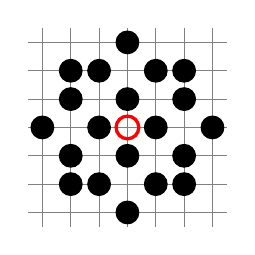
\begin{tikzpicture}[scale=0.36]
\draw[step=1,color=gray] (-3.5,-3.5) grid (3.5,3.5);
\draw[very thick,red] (0, 0) circle (.4);
%%\ draw[very thick] (0,0) circle (2);
%% 1
\filldraw[black] (0,-1) circle (.4);
\filldraw[black] (0,+1) circle (.4);
\filldraw[black] (-1,0) circle (.4);
\filldraw[black] (+1,0) circle (.4);
%% 4
\filldraw[black] (-2,-1) circle (.4);
\filldraw[black] (-2,+1) circle (.4);
\filldraw[black] (-1,-2) circle (.4);
\filldraw[black] (-1,+2) circle (.4);
\filldraw[black] (+1,-2) circle (.4);
\filldraw[black] (+1,+2) circle (.4);
\filldraw[black] (+2,-1) circle (.4);
\filldraw[black] (+2,+1) circle (.4);
%% 5
\filldraw[black] (-2,-2) circle (.4);
\filldraw[black] (-2,+2) circle (.4);
\filldraw[black] (+2,-2) circle (.4);
\filldraw[black] (+2,+2) circle (.4);
%% 6
\filldraw[black] (0,-3) circle (.4);
\filldraw[black] (0,+3) circle (.4);
\filldraw[black] (-3,0) circle (.4);
\filldraw[black] (+3,0) circle (.4);
\end{tikzpicture}
\end{subfigure}
%% ===============================================
\hfill
%% ===============================================
\begin{subfigure}[b]{0.14\textwidth}
\caption{\label{fig:2346nn}}
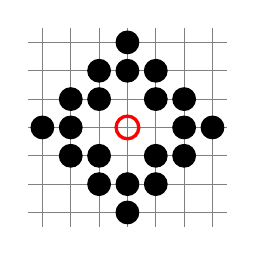
\begin{tikzpicture}[scale=0.36]
\draw[step=1,color=gray] (-3.5,-3.5) grid (3.5,3.5);
\draw[very thick,red] (0, 0) circle (.4);
%%\ draw[very thick] (0,0) circle (2);
%% 2
\filldraw[black] (+1,-1) circle (.4);
\filldraw[black] (+1,+1) circle (.4);
\filldraw[black] (-1,-1) circle (.4);
\filldraw[black] (-1,+1) circle (.4);
%% 3
\filldraw[black] ( 0,-2) circle (.4);
\filldraw[black] ( 0,+2) circle (.4);
\filldraw[black] (-2, 0) circle (.4);
\filldraw[black] (+2, 0) circle (.4);
%% 4
\filldraw[black] (-2,-1) circle (.4);
\filldraw[black] (-2,+1) circle (.4);
\filldraw[black] (-1,-2) circle (.4);
\filldraw[black] (-1,+2) circle (.4);
\filldraw[black] (+1,-2) circle (.4);
\filldraw[black] (+1,+2) circle (.4);
\filldraw[black] (+2,-1) circle (.4);
\filldraw[black] (+2,+1) circle (.4);
%% 6
\filldraw[black] (0,-3) circle (.4);
\filldraw[black] (0,+3) circle (.4);
\filldraw[black] (-3,0) circle (.4);
\filldraw[black] (+3,0) circle (.4);
\end{tikzpicture}
\end{subfigure}
%% ===============================================
\hfill
%% ===============================================
\begin{subfigure}[b]{0.14\textwidth}
\caption{\label{fig:2356nn}}
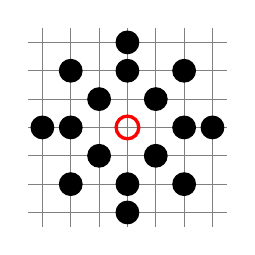
\begin{tikzpicture}[scale=0.36]
\draw[step=1,color=gray] (-3.5,-3.5) grid (3.5,3.5);
\draw[very thick,red] (0, 0) circle (.4);
%%\ draw[very thick] (0,0) circle (2);
%% 2
\filldraw[black] (+1,-1) circle (.4);
\filldraw[black] (+1,+1) circle (.4);
\filldraw[black] (-1,-1) circle (.4);
\filldraw[black] (-1,+1) circle (.4);
%% 3
\filldraw[black] ( 0,-2) circle (.4);
\filldraw[black] ( 0,+2) circle (.4);
\filldraw[black] (-2, 0) circle (.4);
\filldraw[black] (+2, 0) circle (.4);
%% 5
\filldraw[black] (-2,-2) circle (.4);
\filldraw[black] (-2,+2) circle (.4);
\filldraw[black] (+2,-2) circle (.4);
\filldraw[black] (+2,+2) circle (.4);
%% 6
\filldraw[black] (0,-3) circle (.4);
\filldraw[black] (0,+3) circle (.4);
\filldraw[black] (-3,0) circle (.4);
\filldraw[black] (+3,0) circle (.4);
\end{tikzpicture}
\end{subfigure}
%% ===============================================
\hfill
%% ===============================================
\begin{subfigure}[b]{0.14\textwidth}
\caption{\label{fig:2456nn}}
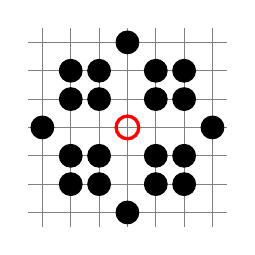
\begin{tikzpicture}[scale=0.36]
\draw[step=1,color=gray] (-3.5,-3.5) grid (3.5,3.5);
\draw[very thick,red] (0, 0) circle (.4);
%% 2
\filldraw[black] (+1,-1) circle (.4);
\filldraw[black] (+1,+1) circle (.4);
\filldraw[black] (-1,-1) circle (.4);
\filldraw[black] (-1,+1) circle (.4);
%% 4
\filldraw[black] (-2,-1) circle (.4);
\filldraw[black] (-2,+1) circle (.4);
\filldraw[black] (-1,-2) circle (.4);
\filldraw[black] (-1,+2) circle (.4);
\filldraw[black] (+1,-2) circle (.4);
\filldraw[black] (+1,+2) circle (.4);
\filldraw[black] (+2,-1) circle (.4);
\filldraw[black] (+2,+1) circle (.4);
%% 5
\filldraw[black] (-2,-2) circle (.4);
\filldraw[black] (-2,+2) circle (.4);
\filldraw[black] (+2,-2) circle (.4);
\filldraw[black] (+2,+2) circle (.4);
%% 6
\filldraw[black] (0,-3) circle (.4);
\filldraw[black] (0,+3) circle (.4);
\filldraw[black] (-3,0) circle (.4);
\filldraw[black] (+3,0) circle (.4);
\end{tikzpicture}
\end{subfigure}
%% ===============================================
\hfill
%% ===============================================
\begin{subfigure}[b]{0.14\textwidth}
\caption{\label{fig:3456nn}}
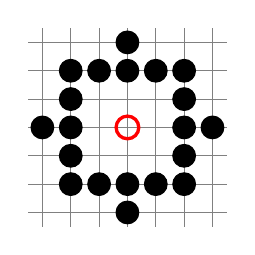
\begin{tikzpicture}[scale=0.36]
\draw[step=1,color=gray] (-3.5,-3.5) grid (3.5,3.5);
\draw[very thick,red] (0, 0) circle (.4);
%% 3
\filldraw[black] ( 0,-2) circle (.4);
\filldraw[black] ( 0,+2) circle (.4);
\filldraw[black] (-2, 0) circle (.4);
\filldraw[black] (+2, 0) circle (.4);
%% 4
\filldraw[black] (-2,-1) circle (.4);
\filldraw[black] (-2,+1) circle (.4);
\filldraw[black] (-1,-2) circle (.4);
\filldraw[black] (-1,+2) circle (.4);
\filldraw[black] (+1,-2) circle (.4);
\filldraw[black] (+1,+2) circle (.4);
\filldraw[black] (+2,-1) circle (.4);
\filldraw[black] (+2,+1) circle (.4);
%% 5
\filldraw[black] (-2,-2) circle (.4);
\filldraw[black] (-2,+2) circle (.4);
\filldraw[black] (+2,-2) circle (.4);
\filldraw[black] (+2,+2) circle (.4);
%% 6
\filldraw[black] (0,-3) circle (.4);
\filldraw[black] (0,+3) circle (.4);
\filldraw[black] (-3,0) circle (.4);
\filldraw[black] (+3,0) circle (.4);
\end{tikzpicture}
\end{subfigure}
%% ===============================================
\hfill
%% ===============================================
\begin{subfigure}[b]{0.14\textwidth}
\caption{\label{fig:12346nn}}
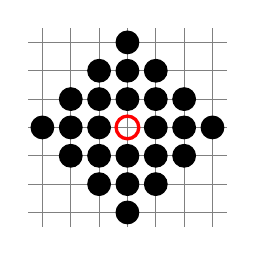
\begin{tikzpicture}[scale=0.36]
\draw[step=1,color=gray] (-3.5,-3.5) grid (3.5,3.5);
\draw[very thick,red] (0, 0) circle (.4);
%%\ draw[very thick] (0,0) circle (2);
%% 1
\filldraw[black] (0,-1) circle (.4);
\filldraw[black] (0,+1) circle (.4);
\filldraw[black] (-1,0) circle (.4);
\filldraw[black] (+1,0) circle (.4);
%% 2
\filldraw[black] (+1,-1) circle (.4);
\filldraw[black] (+1,+1) circle (.4);
\filldraw[black] (-1,-1) circle (.4);
\filldraw[black] (-1,+1) circle (.4);
%% 3
\filldraw[black] ( 0,-2) circle (.4);
\filldraw[black] ( 0,+2) circle (.4);
\filldraw[black] (-2, 0) circle (.4);
\filldraw[black] (+2, 0) circle (.4);
%% 4
\filldraw[black] (-2,-1) circle (.4);
\filldraw[black] (-2,+1) circle (.4);
\filldraw[black] (-1,-2) circle (.4);
\filldraw[black] (-1,+2) circle (.4);
\filldraw[black] (+1,-2) circle (.4);
\filldraw[black] (+1,+2) circle (.4);
\filldraw[black] (+2,-1) circle (.4);
\filldraw[black] (+2,+1) circle (.4);
%% 6
\filldraw[black] (0,-3) circle (.4);
\filldraw[black] (0,+3) circle (.4);
\filldraw[black] (-3,0) circle (.4);
\filldraw[black] (+3,0) circle (.4);
\end{tikzpicture}
\end{subfigure}
%% ===============================================
\hfill
%% ===============================================
\begin{subfigure}[b]{0.14\textwidth}
\caption{\label{fig:12356nn}}
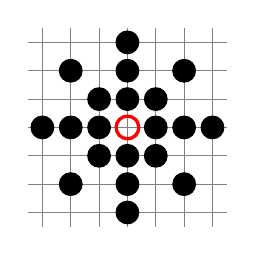
\begin{tikzpicture}[scale=0.36]
\draw[step=1,color=gray] (-3.5,-3.5) grid (3.5,3.5);
\draw[very thick,red] (0, 0) circle (.4);
%%\ draw[very thick] (0,0) circle (2);
%% 1
\filldraw[black] (0,-1) circle (.4);
\filldraw[black] (0,+1) circle (.4);
\filldraw[black] (-1,0) circle (.4);
\filldraw[black] (+1,0) circle (.4);
%% 2
\filldraw[black] (+1,-1) circle (.4);
\filldraw[black] (+1,+1) circle (.4);
\filldraw[black] (-1,-1) circle (.4);
\filldraw[black] (-1,+1) circle (.4);
%% 3
\filldraw[black] ( 0,-2) circle (.4);
\filldraw[black] ( 0,+2) circle (.4);
\filldraw[black] (-2, 0) circle (.4);
\filldraw[black] (+2, 0) circle (.4);
%% 5
\filldraw[black] (-2,-2) circle (.4);
\filldraw[black] (-2,+2) circle (.4);
\filldraw[black] (+2,-2) circle (.4);
\filldraw[black] (+2,+2) circle (.4);
%% 6
\filldraw[black] (0,-3) circle (.4);
\filldraw[black] (0,+3) circle (.4);
\filldraw[black] (-3,0) circle (.4);
\filldraw[black] (+3,0) circle (.4);
\end{tikzpicture}
\end{subfigure}
%% ===============================================
\hfill
%% ===============================================
\begin{subfigure}[b]{0.14\textwidth}
\caption{\label{fig:12456nn}}
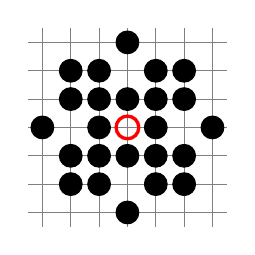
\begin{tikzpicture}[scale=0.36]
\draw[step=1,color=gray] (-3.5,-3.5) grid (3.5,3.5);
\draw[very thick,red] (0, 0) circle (.4);
%%\ draw[very thick] (0,0) circle (2);
%% 1
\filldraw[black] (0,-1) circle (.4);
\filldraw[black] (0,+1) circle (.4);
\filldraw[black] (-1,0) circle (.4);
\filldraw[black] (+1,0) circle (.4);
%% 2
\filldraw[black] (+1,-1) circle (.4);
\filldraw[black] (+1,+1) circle (.4);
\filldraw[black] (-1,-1) circle (.4);
\filldraw[black] (-1,+1) circle (.4);
%% 4
\filldraw[black] (-2,-1) circle (.4);
\filldraw[black] (-2,+1) circle (.4);
\filldraw[black] (-1,-2) circle (.4);
\filldraw[black] (-1,+2) circle (.4);
\filldraw[black] (+1,-2) circle (.4);
\filldraw[black] (+1,+2) circle (.4);
\filldraw[black] (+2,-1) circle (.4);
\filldraw[black] (+2,+1) circle (.4);
%% 5
\filldraw[black] (-2,-2) circle (.4);
\filldraw[black] (-2,+2) circle (.4);
\filldraw[black] (+2,-2) circle (.4);
\filldraw[black] (+2,+2) circle (.4);
%% 6
\filldraw[black] (0,-3) circle (.4);
\filldraw[black] (0,+3) circle (.4);
\filldraw[black] (-3,0) circle (.4);
\filldraw[black] (+3,0) circle (.4);
\end{tikzpicture}
\end{subfigure}
%% ===============================================
\hfill
%% ===============================================
\begin{subfigure}[b]{0.14\textwidth}
\caption{\label{fig:13456nn}}
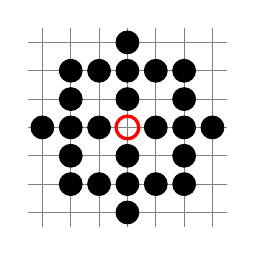
\begin{tikzpicture}[scale=0.36]
\draw[step=1,color=gray] (-3.5,-3.5) grid (3.5,3.5);
\draw[very thick,red] (0, 0) circle (.4);
%%\ draw[very thick] (0,0) circle (2);
%% 1
\filldraw[black] (0,-1) circle (.4);
\filldraw[black] (0,+1) circle (.4);
\filldraw[black] (-1,0) circle (.4);
\filldraw[black] (+1,0) circle (.4);
%% 3
\filldraw[black] ( 0,-2) circle (.4);
\filldraw[black] ( 0,+2) circle (.4);
\filldraw[black] (-2, 0) circle (.4);
\filldraw[black] (+2, 0) circle (.4);
%% 4
\filldraw[black] (-2,-1) circle (.4);
\filldraw[black] (-2,+1) circle (.4);
\filldraw[black] (-1,-2) circle (.4);
\filldraw[black] (-1,+2) circle (.4);
\filldraw[black] (+1,-2) circle (.4);
\filldraw[black] (+1,+2) circle (.4);
\filldraw[black] (+2,-1) circle (.4);
\filldraw[black] (+2,+1) circle (.4);
%% 5
\filldraw[black] (-2,-2) circle (.4);
\filldraw[black] (-2,+2) circle (.4);
\filldraw[black] (+2,-2) circle (.4);
\filldraw[black] (+2,+2) circle (.4);
%% 6
\filldraw[black] (0,-3) circle (.4);
\filldraw[black] (0,+3) circle (.4);
\filldraw[black] (-3,0) circle (.4);
\filldraw[black] (+3,0) circle (.4);
\end{tikzpicture}
\end{subfigure}
%% ===============================================
\hfill
%% ===============================================
\begin{subfigure}[b]{0.14\textwidth}
\caption{\label{fig:23456nn}}
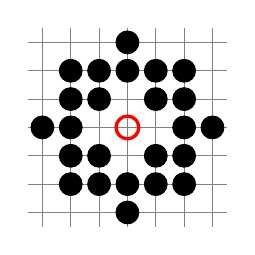
\begin{tikzpicture}[scale=0.36]
\draw[step=1,color=gray] (-3.5,-3.5) grid (3.5,3.5);
\draw[very thick,red] (0, 0) circle (.4);
%%\ draw[very thick] (0,0) circle (2);
%% 2
\filldraw[black] (+1,-1) circle (.4);
\filldraw[black] (+1,+1) circle (.4);
\filldraw[black] (-1,-1) circle (.4);
\filldraw[black] (-1,+1) circle (.4);
%% 3
\filldraw[black] ( 0,-2) circle (.4);
\filldraw[black] ( 0,+2) circle (.4);
\filldraw[black] (-2, 0) circle (.4);
\filldraw[black] (+2, 0) circle (.4);
%% 4
\filldraw[black] (-2,-1) circle (.4);
\filldraw[black] (-2,+1) circle (.4);
\filldraw[black] (-1,-2) circle (.4);
\filldraw[black] (-1,+2) circle (.4);
\filldraw[black] (+1,-2) circle (.4);
\filldraw[black] (+1,+2) circle (.4);
\filldraw[black] (+2,-1) circle (.4);
\filldraw[black] (+2,+1) circle (.4);
%% 5
\filldraw[black] (-2,-2) circle (.4);
\filldraw[black] (-2,+2) circle (.4);
\filldraw[black] (+2,-2) circle (.4);
\filldraw[black] (+2,+2) circle (.4);
%% 6
\filldraw[black] (0,-3) circle (.4);
\filldraw[black] (0,+3) circle (.4);
\filldraw[black] (-3,0) circle (.4);
\filldraw[black] (+3,0) circle (.4);
\end{tikzpicture}
\end{subfigure}
%% ===============================================
\hfill
%% ===============================================
\begin{subfigure}[b]{0.14\textwidth}
\caption{\label{fig:123456nn}}
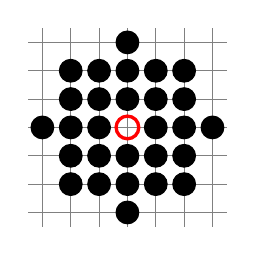
\begin{tikzpicture}[scale=0.36]
\draw[step=1,color=gray] (-3.5,-3.5) grid (3.5,3.5);
\draw[very thick,red] (0, 0) circle (.4);
%%\ draw[very thick] (0,0) circle (2);
%% 1
\filldraw[black] (0,-1) circle (.4);
\filldraw[black] (0,+1) circle (.4);
\filldraw[black] (-1,0) circle (.4);
\filldraw[black] (+1,0) circle (.4);
%% 2
\filldraw[black] (+1,-1) circle (.4);
\filldraw[black] (+1,+1) circle (.4);
\filldraw[black] (-1,-1) circle (.4);
\filldraw[black] (-1,+1) circle (.4);
%% 3
\filldraw[black] ( 0,-2) circle (.4);
\filldraw[black] ( 0,+2) circle (.4);
\filldraw[black] (-2, 0) circle (.4);
\filldraw[black] (+2, 0) circle (.4);
%% 4
\filldraw[black] (-2,-1) circle (.4);
\filldraw[black] (-2,+1) circle (.4);
\filldraw[black] (-1,-2) circle (.4);
\filldraw[black] (-1,+2) circle (.4);
\filldraw[black] (+1,-2) circle (.4);
\filldraw[black] (+1,+2) circle (.4);
\filldraw[black] (+2,-1) circle (.4);
\filldraw[black] (+2,+1) circle (.4);
%% 5
\filldraw[black] (-2,-2) circle (.4);
\filldraw[black] (-2,+2) circle (.4);
\filldraw[black] (+2,-2) circle (.4);
\filldraw[black] (+2,+2) circle (.4);
%% 6
\filldraw[black] (0,-3) circle (.4);
\filldraw[black] (0,+3) circle (.4);
\filldraw[black] (-3,0) circle (.4);
\filldraw[black] (+3,0) circle (.4);
\end{tikzpicture}
\end{subfigure}
%% ===============================================
\caption{\label{fig:sq-neighbourhoods}(Color online). Shapes of neighborhoods on square lattice combined with basics neighborhoods presented in \Cref{fig:sq-basic-neighbourhoods} and containing sites from the sixth coordination zone (\Cref{fig:sq-6nn}).
%% -----------------------------------------------
\subref{fig:16nn}     \textsc{sq-1,6},
\subref{fig:26nn}     \textsc{sq-2,6},
\subref{fig:36nn}     \textsc{sq-3,6},
\subref{fig:46nn}     \textsc{sq-4,6},
\subref{fig:56nn}     \textsc{sq-5,6},
%% -----------------------------------------------
\subref{fig:126nn}    \textsc{sq-1,2,6},
\subref{fig:136nn}    \textsc{sq-1,3,6},
\subref{fig:146nn}    \textsc{sq-1,4,6},
\subref{fig:156nn}    \textsc{sq-1,5,6},
\subref{fig:236nn}    \textsc{sq-2,3,6},
\subref{fig:246nn}    \textsc{sq-2,4,6},
\subref{fig:256nn}    \textsc{sq-2,5,6},
\subref{fig:346nn}    \textsc{sq-3,4,6},
\subref{fig:356nn}    \textsc{sq-3,5,6},
\subref{fig:456nn}    \textsc{sq-4,5,6},
%% -----------------------------------------------
\subref{fig:1236nn}   \textsc{sq-1,2,3,6},
\subref{fig:1246nn}   \textsc{sq-1,2,4,6},
\subref{fig:1256nn}   \textsc{sq-1,2,5,6},
\subref{fig:1346nn}   \textsc{sq-1,3,4,6},
\subref{fig:1356nn}   \textsc{sq-1,3,5,6},
\subref{fig:1456nn}   \textsc{sq-1,4,5,6},
\subref{fig:2346nn}   \textsc{sq-2,3,4,6},
\subref{fig:2356nn}   \textsc{sq-2,3,5,6},
\subref{fig:2456nn}   \textsc{sq-2,4,5,6},
\subref{fig:3456nn}   \textsc{sq-3,4,5,6},
%% -----------------------------------------------
\subref{fig:12346nn}  \textsc{sq-1,2,3,4,6},
\subref{fig:12356nn}  \textsc{sq-1,2,3,5,6},
\subref{fig:12456nn}  \textsc{sq-1,2,4,5,6},
\subref{fig:13456nn}  \textsc{sq-1,3,4,5,6},
\subref{fig:23456nn}  \textsc{sq-2,3,4,5,6},
%% -----------------------------------------------
\subref{fig:123456nn} \textsc{sq-1,2,3,4,5,6}}
%% ===============================================